% --- Sequence and context parallelism ---
\begin{frame}{What Tensor Parallelism Leaves Replicated}
  \begin{itemize}\scriptsize\itemsep0.05em
    \item[\textcolor{red}{$\blacktriangleright$}] Tensor parallelism shards the attention and MLP interiors, but the regions \emph{between} them --- LayerNorm, dropout, and the residual adds --- are elementwise. They need no weights, so Megatron leaves them replicated on all $t$ ranks.
    \item[\textcolor{red}{$\blacktriangleright$}] Those regions still hold activations. Writing the per-layer activation memory with tensor parallelism of degree $t$:
      \[
        s\,b\,h\!\left(10 + \frac{24}{t} + \frac{5as}{ht}\right)
      \]
      the $10$ is the stubborn part: it does not shrink no matter how large $t$ becomes.
    \item[\textcolor{red}{$\blacktriangleright$}] \textbf{Sequence parallelism} shards those regions along the \textbf{sequence} dimension. Each rank owns $s/t$ positions of the LayerNorm and dropout tensors, which is legal precisely because those operations are independent across positions.
  \end{itemize}
  \vspace{0.04em}
  \centering
  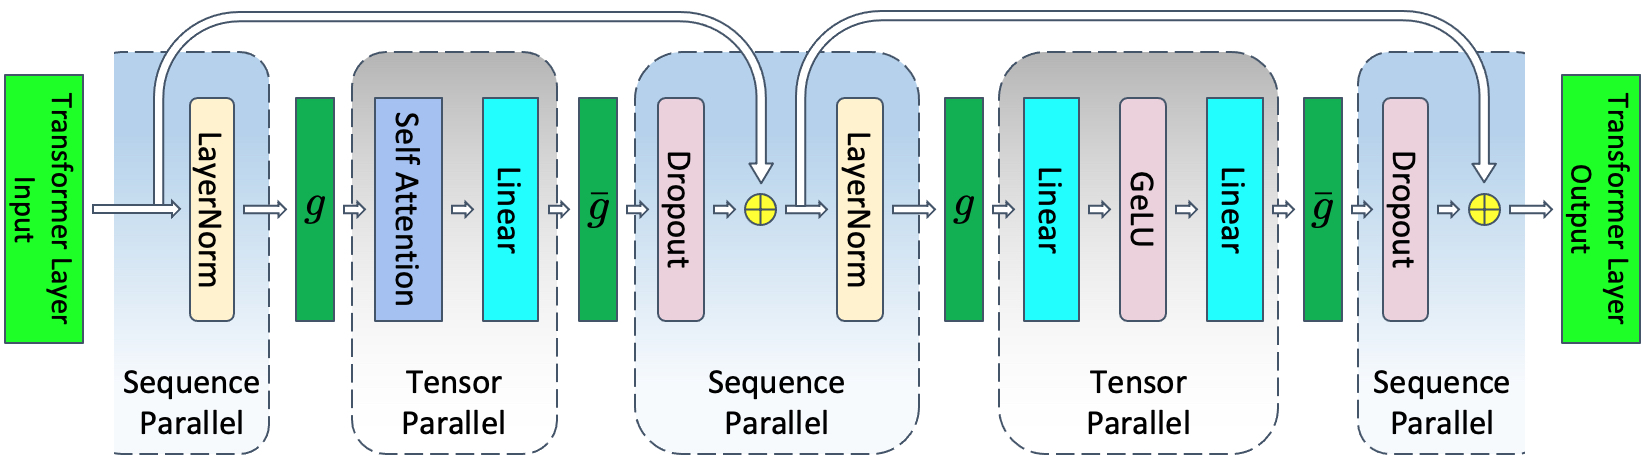
\includegraphics[width=0.92\textwidth,height=0.27\textheight,keepaspectratio]{images/distributed-training/korthikanti_fig5_tensor_and_sequence_parallel_layer.jpg}\\[0.15em]
  {\scriptsize A transformer layer with tensor \emph{and} sequence parallelism. $g$ is an all-gather forward and reduce-scatter backward; $\bar{g}$ is the conjugate. Korthikanti et al., \href{https://arxiv.org/abs/2205.05198v1}{arXiv:2205.05198v1}, Figure 5.}
\end{frame}

\begin{frame}{Sequence Parallelism Costs Nothing Extra}
  \begin{columns}[T,onlytextwidth]
    \column{0.5\textwidth}
      \begin{itemize}\footnotesize\itemsep0.3em
        \item[\textcolor{red}{$\blacktriangleright$}] The one all-reduce at each tensor-parallel boundary is \textbf{replaced} by an all-gather (entering the region) and a reduce-scatter (leaving it).
        \item[\textcolor{red}{$\blacktriangleright$}] Since an all-reduce \emph{is} a reduce-scatter plus an all-gather, the communication volume is \textbf{unchanged}. Sequence parallelism is a pure memory win. Per layer it gives
          \[
            \frac{s\,b\,h}{t}\left(34 + \frac{5as}{h}\right),
          \]
          the full activation term divided cleanly by $t$.
        \item[\textcolor{red}{$\blacktriangleright$}] Add \textbf{selective activation recomputation} --- recompute only the attention softmax and dropout region, cheap in FLOPs but huge in bytes --- and the model's activations collapse to $34sbhL/t$.
        \item[\textcolor{red}{$\blacktriangleright$}] Together: a \textbf{5$\times$} memory reduction that recovers over \textbf{90\%} of the time lost to full recomputation. On a 530B model across 2240 A100s this raised model FLOPs utilisation from 42.1\% to \textbf{54.2\%}.
      \end{itemize}
    \column{0.48\textwidth}
      \centering
      \vspace{0.6em}
      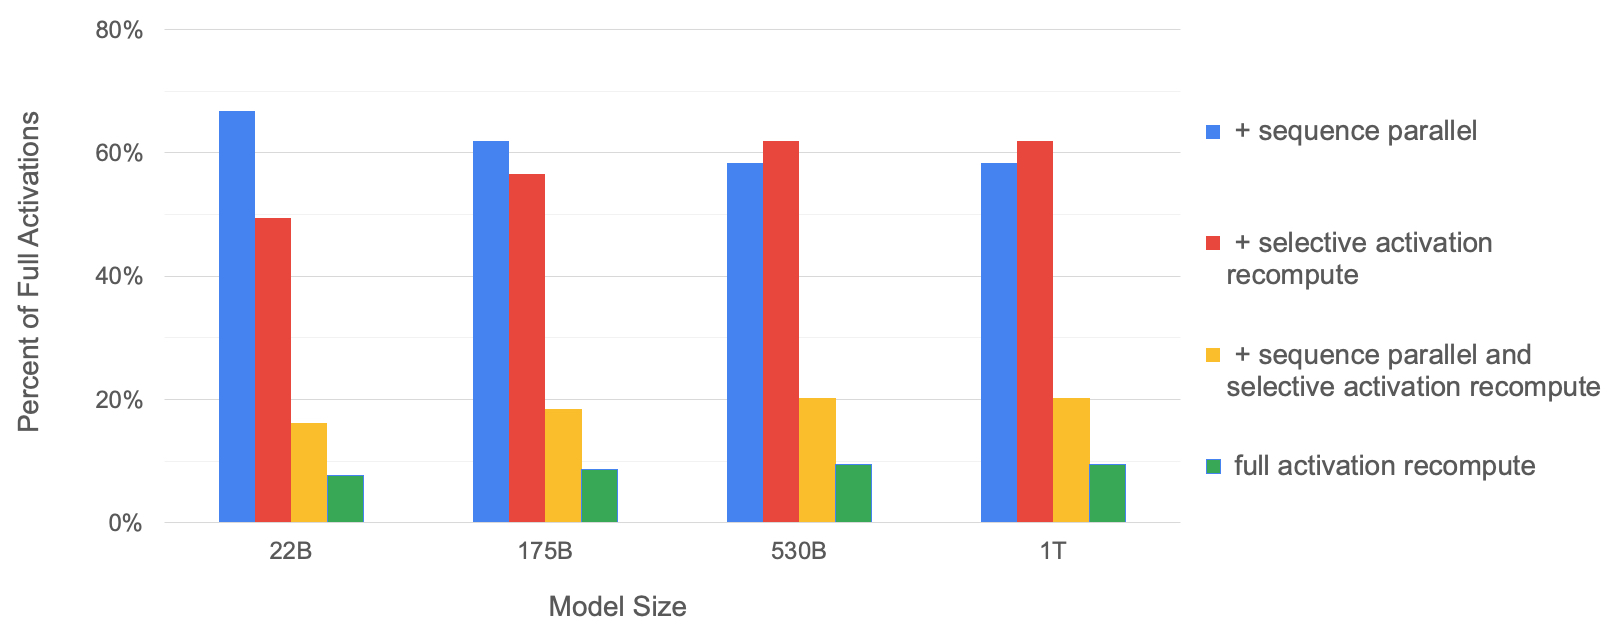
\includegraphics[width=\linewidth,height=0.55\textheight,keepaspectratio]{images/distributed-training/korthikanti_fig7_percentage_of_full_activations.jpg}\\[0.2em]
      {\scriptsize Activation memory as a percentage of the tensor-parallel baseline. Korthikanti et al., \href{https://arxiv.org/abs/2205.05198v1}{arXiv:2205.05198v1}, Figure 7.}
  \end{columns}
\end{frame}

\begin{frame}[allowframebreaks]{Two Different Things Called ``Sequence Parallelism''}
  \begin{itemize}\itemsep0.45em
    \item[\textcolor{red}{$\blacktriangleright$}] This is a genuine naming collision in the literature, and it causes real confusion when reading configuration files.
    \item[\textcolor{red}{$\blacktriangleright$}] \textbf{Megatron sequence parallelism} (previous two slides) splits the \emph{non-attention} regions along the sequence, \emph{inside} an existing tensor-parallel group. It does not increase the number of GPUs you can use; it reduces memory at fixed $t$. Attention still sees the whole sequence.
    \item[\textcolor{red}{$\blacktriangleright$}] \textbf{Context parallelism} splits the sequence across a \emph{separate} parallel group and makes attention itself distributed. Each device holds $s/c$ positions of $Q$, $K$, and $V$, and the attention computation must somehow see the other devices' keys and values. This \emph{is} a new axis: it raises the maximum trainable context length in proportion to the device count.
    \item[\textcolor{red}{$\blacktriangleright$}] Two mechanisms dominate:
      \begin{itemize}\itemsep0.2em\footnotesize
        \item \textbf{Ring Attention} (Liu et al.): pass key/value blocks around a ring of devices, overlapping the transfer with blockwise attention compute.
        \item \textbf{DeepSpeed-Ulysses} (Jacobs et al.): use an all-to-all to switch from a sequence-sharded layout to a head-sharded layout for the attention itself, then switch back. Reported 2.5$\times$ speed at 4$\times$ the sequence length of the prior state of the art.
      \end{itemize}
    \item[\textcolor{red}{$\blacktriangleright$}] Both are \emph{exact}: they compute the same attention as a single device would, unlike sparse or windowed approximations.
  \end{itemize}
\end{frame}

\begin{frame}{Ring Attention}
  \begin{columns}[T,onlytextwidth]
    \column{0.47\textwidth}
      \begin{itemize}\footnotesize\itemsep0.3em
        \item[\textcolor{red}{$\blacktriangleright$}] \textbf{The enabling property:} attention between one query block and a set of key/value blocks can be accumulated in \emph{any order}, provided the running softmax statistics are rescaled correctly --- the same online-softmax trick FlashAttention uses inside one GPU.
        \item[\textcolor{red}{$\blacktriangleright$}] So arrange the devices in a ring. Each keeps one query block permanently while key/value blocks rotate: a device computes attention against the block it holds while \textbf{sending that block onward} and \textbf{receiving the next from its predecessor}.
        \item[\textcolor{red}{$\blacktriangleright$}] If blockwise compute takes at least as long as one block transfer, communication is \textbf{completely hidden}: zero overhead, no approximation.
        \item[\textcolor{red}{$\blacktriangleright$}] That condition sets a minimum sequence length per device, fixed by the ratio of device FLOPs to interconnect bandwidth. Slower links need bigger blocks.
      \end{itemize}
    \column{0.5\textwidth}
      \centering
      \vspace{0.4em}
      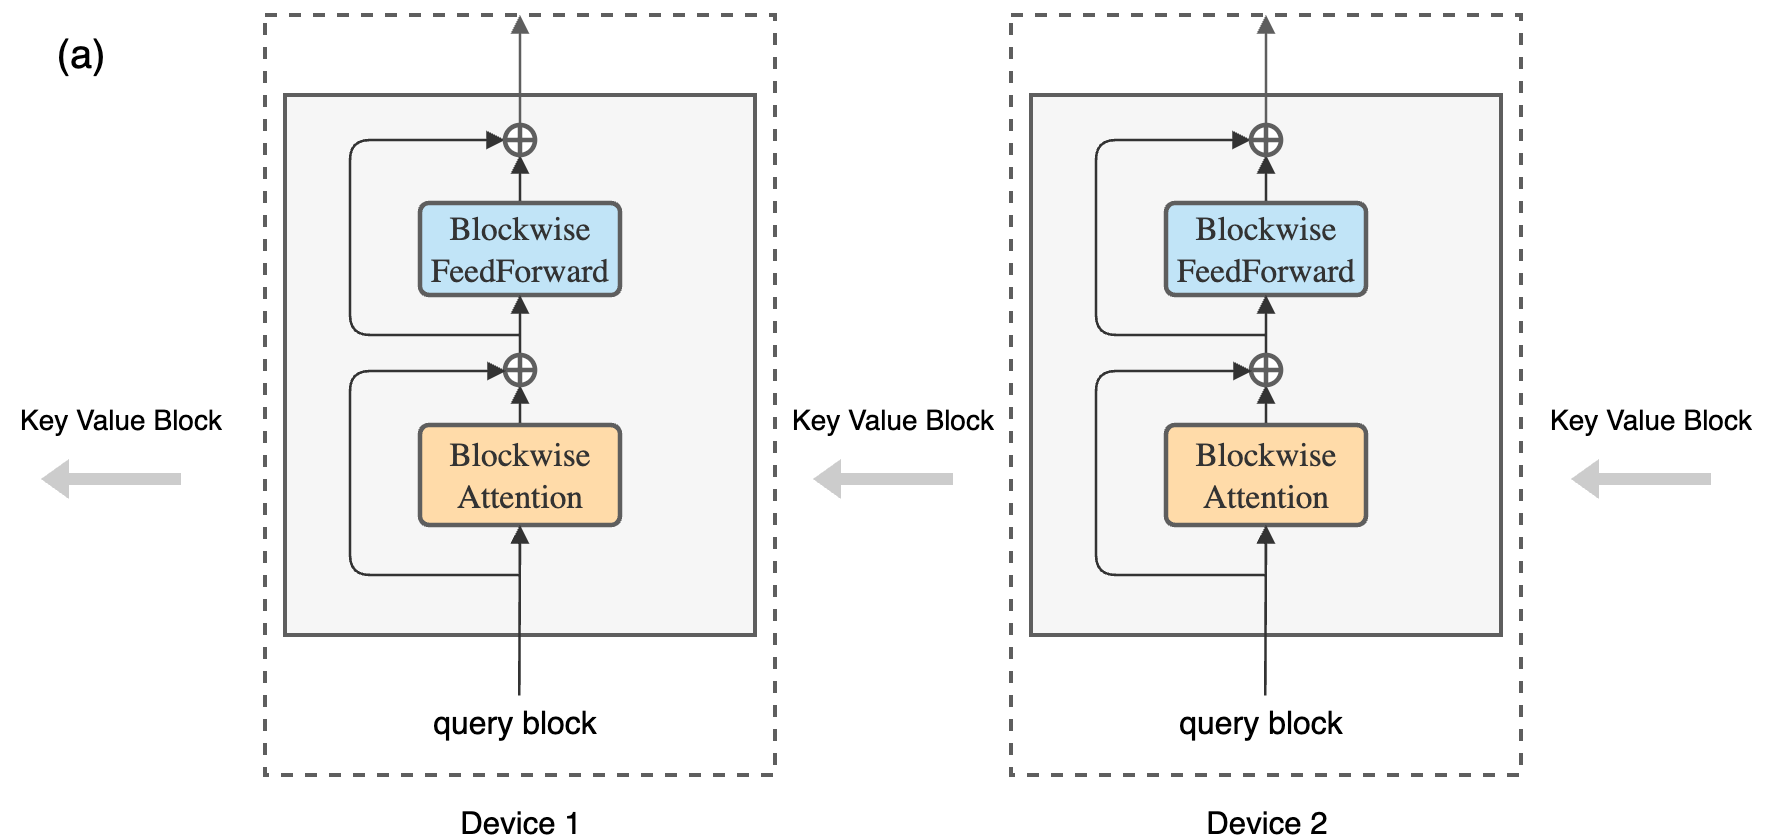
\includegraphics[width=\linewidth,height=0.44\textheight,keepaspectratio]{images/distributed-training/ring_attention_fig2a_kv_blocks_traverse_ring.png}\\[0.2em]
      {\scriptsize Key/value blocks traverse a ring of hosts while each host keeps its own query block. Liu, Zaharia \& Abbeel, ``Ring Attention with Blockwise Transformers for Near-Infinite Context,'' \href{https://arxiv.org/abs/2310.01889v4}{arXiv:2310.01889v4}, Figure 2(a).}
  \end{columns}
\end{frame}

\begin{frame}{How Million-Token Contexts Get Trained}
  \begin{columns}[T,onlytextwidth]
    \column{0.5\textwidth}
      \begin{itemize}\footnotesize\itemsep0.3em
        \item[\textcolor{red}{$\blacktriangleright$}] The headline claim is a scaling statement, not a constant-factor one: Ring Attention supports sequences ``up to \textbf{device count times longer}'' than the memory-efficient baselines.
        \item[\textcolor{red}{$\blacktriangleright$}] The intuition: memory-efficient attention already removed the $O(s^2)$ term on one device, leaving $O(s)$. Sharding the sequence over $c$ devices divides \emph{that} by $c$, so nothing grows faster than linearly and the ceiling moves with the cluster.
        \item[\textcolor{red}{$\blacktriangleright$}] This is the machinery behind million-token context windows --- and the reason they are expensive: the \emph{compute} stays quadratic even when the \emph{memory} does not.
        \item[\textcolor{red}{$\blacktriangleright$}] You will meet it as \texttt{context\_parallel\_size} (Megatron-LM, NeMo) or \texttt{sequence\_parallel\_size} (DeepSpeed), composed with $t$, $p$, and $d$.
      \end{itemize}
    \column{0.48\textwidth}
      \centering
      \vspace{0.5em}
      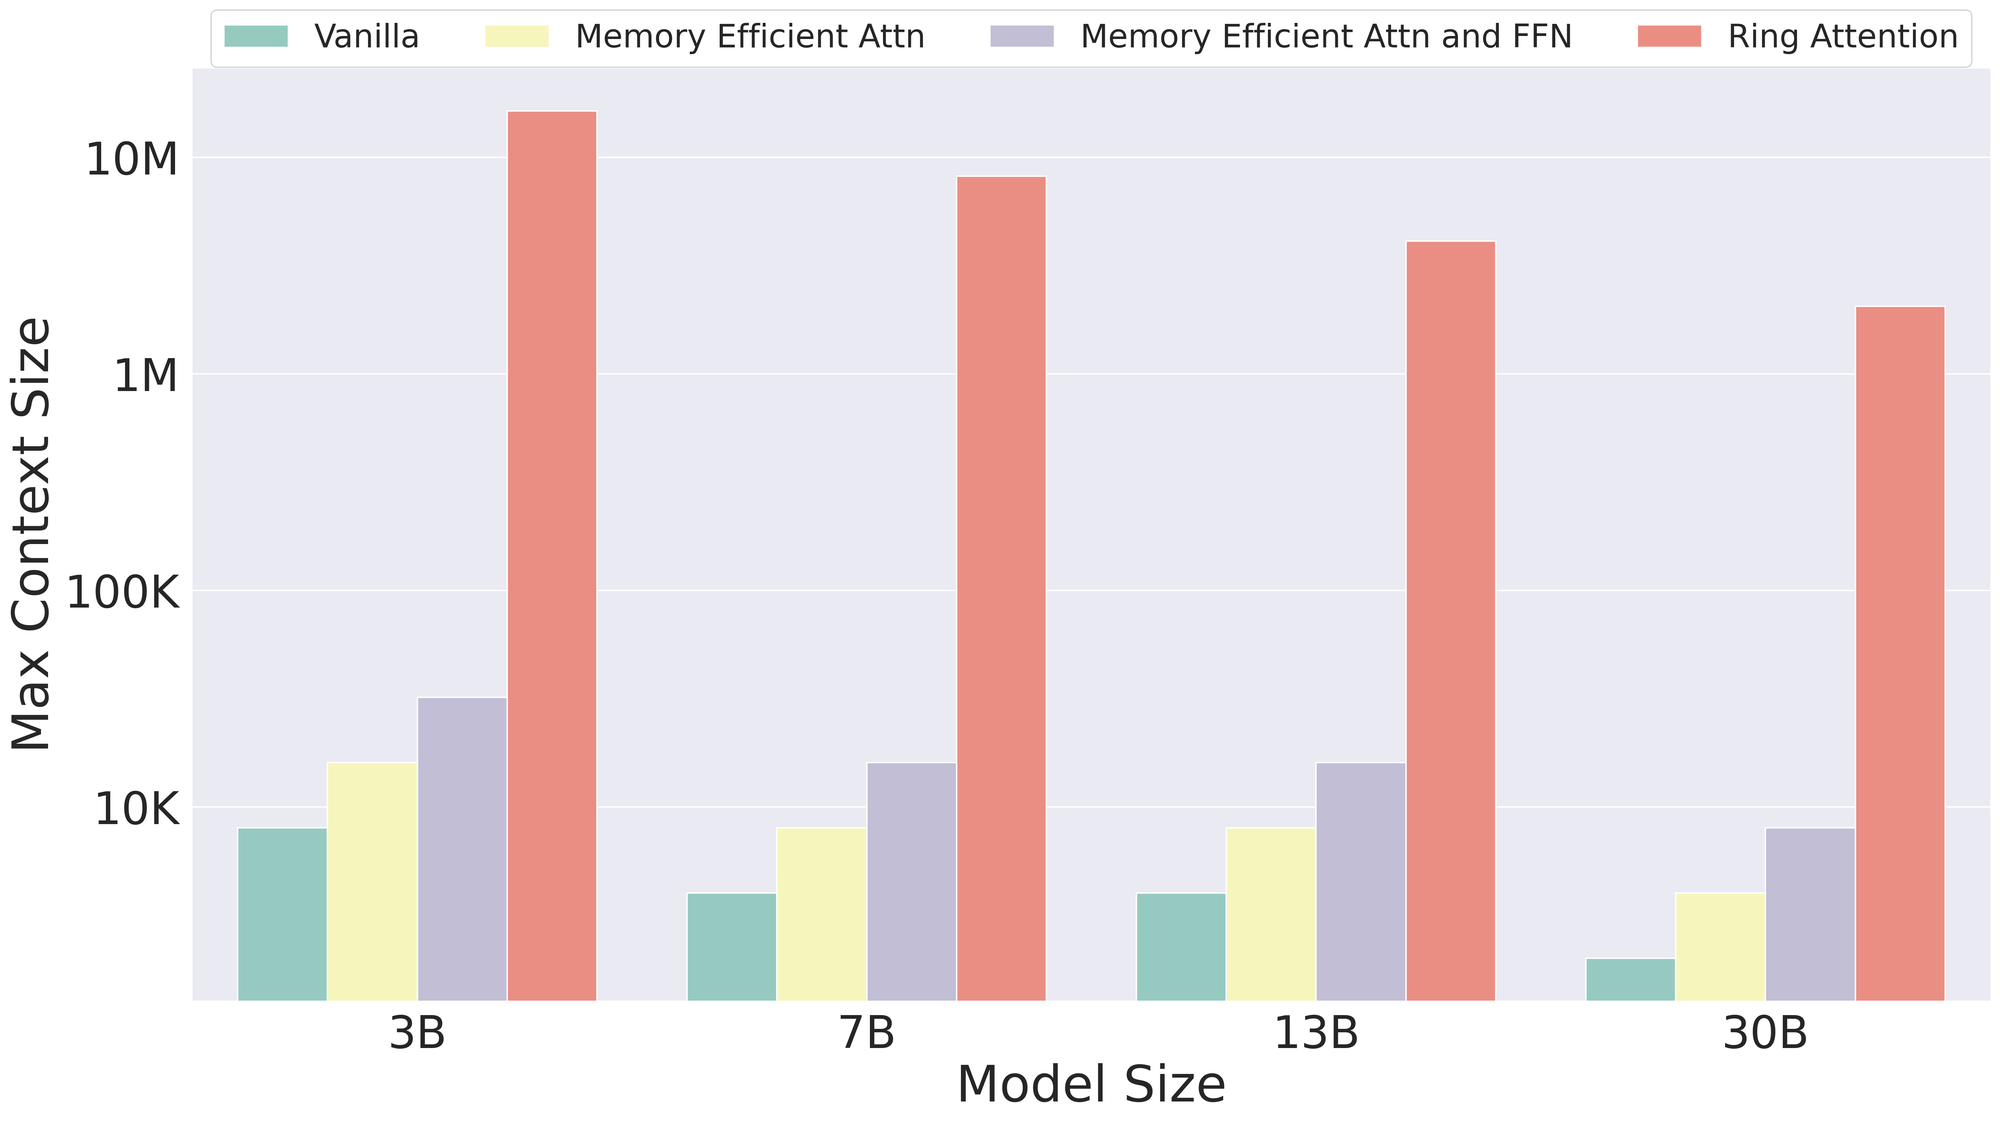
\includegraphics[width=\linewidth,height=0.5\textheight,keepaspectratio]{images/distributed-training/ring_attention_fig1_max_context_length.png}\\[0.2em]
      {\scriptsize Maximum context length in end-to-end training on TPUv4-1024, against vanilla, memory-efficient, and blockwise-parallel transformers. Liu, Zaharia \& Abbeel, \href{https://arxiv.org/abs/2310.01889v4}{arXiv:2310.01889v4}, Figure 1.}
  \end{columns}
\end{frame}
